\chapter{ĐỘNG HỌC CỦA CHUYỂN ĐỘNG TRÒN}
\begin{tomtat}
	\subsubsection{Định nghĩa radian. Số đo cung tròn theo góc}
	\paragraph{Định nghĩa radian}
	\immini{Radian là đơn vị đo độ lớn của một góc: 1 radian (\SI{1}{\radian}) là góc chắn cung có chiều dài bằng bán kính đường tròn.
	$$\SI{1}{\radian}=\dfrac{\SI{180}{\degree}}{\pi}\approx\SI{57.2958}{\degree}.$$
	}{\vspace{-0.75cm}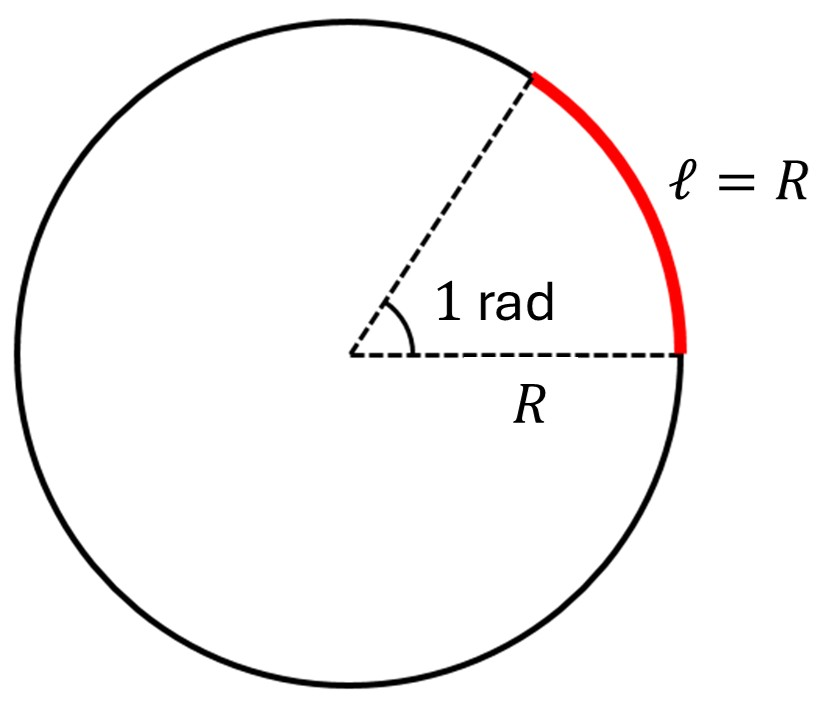
\includegraphics[scale=0.3]{figs/CHUONG8-1}}
	\begin{boxdn}
		\textbf{Hệ thức chuyển đổi đơn vị từ độ sang radian:}
		$$\alpha_{\si{\radian}}=\alpha^{\si{\degree}}\cdot\dfrac{\pi}{\SI{180}{\degree}}.$$
		\textbf{Hệ thức chuyển đổi đơn vị từ radian sang độ:}
		$$\alpha^{\si{\degree}}=\alpha_{\si{\radian}}\cdot\dfrac{\SI{180}{\degree}}{\pi}.$$
	\end{boxdn}
	\paragraph{Số đo cung tròn theo góc}
	\begin{boxdn}
		Khi góc chắn cung có số đo là $\alpha$ (\si{\radian}) thì chiều dài cung tròn sẽ bằng:
		$$\ell=\alpha\cdot R.$$
	\end{boxdn}
	\subsubsection{Tốc độ trong chuyển động tròn}
	\paragraph{Chuyển động tròn}
	\begin{dn}
		Chuyển động tròn là chuyển động có quỹ đạo là một đường tròn.
	\end{dn}
	\paragraph{Tốc độ góc}
	\begin{dn}
		Tốc độ góc là đại lượng đặc trưng cho tính nhanh chậm của chuyển động quay.\\
		Tốc độ góc được xác định bằng góc quay được bởi bán kính trong một đơn vị thời gian:
		$$\omega=\dfrac{\Delta \alpha}{\Delta t}.$$
	\end{dn}
	Trong đó:
	\begin{itemize}
		\item $\omega$: tốc độ góc (\si{\radian/\second});
		\item $\Delta \alpha$: góc quét (\si{\radian});
		\item $\Delta t$: thời gian (\si{\second}).
	\end{itemize}
	\begin{note}
		Khi vật chuyển động tròn đều, $\omega$ là hằng số. Trong các khoảng thời gian bằng nhau, góc quay cũng bằng nhau.
	\end{note}
	\paragraph{Vận tốc trong chuyển động tròn}
	\begin{boxdn}
		Tốc độ của chất điểm chuyển động tròn được tính bằng quãng đường mà chất điểm đi được trong một đơn vị thời gian:
		$$v=\dfrac{s}{\Delta t}=\omega\cdot R.$$
	\end{boxdn}
	Trong chuyển động tròn đều, vector vận tốc $\vec{v}$ có:
	\begin{itemize}
		\item Phương: tiếp tuyến quỹ đạo (đường tròn);
		\item Chiều: cùng chiều chuyển động;
		\item Độ lớn: không đổi $v=\omega\cdot R$.
	\end{itemize}
	\paragraph{Chu kì và tần số}
	\begin{dn}
		Chu kì là thời gian vật thực hiện hết một vòng quay:
		$$T=\dfrac{\Delta t}{N}.$$
	\end{dn}
	Trong đó:
	\begin{itemize}
		\item $	T$: chu kì quay (\si{\second});
		\item $\Delta t$: thời gian chuyển động (\si{\second});
		\item $N$: số vòng quay.
	\end{itemize}
	\begin{dn}
		Tần số là số vòng quay trong một đơn vị thời gian:
		$$f=\dfrac{N}{\Delta t}.$$
		
	\end{dn}
	Đơn vị của $f$ là \si{\text{vòng}/\second} hoặc $\si{\hertz}$ (hertz).
	\begin{boxdn}
		\textbf{Mối liên hệ giữa $\omega$, $T$, $f$:}
		$$\omega=\dfrac{2\pi}{T}=2\pi f.$$
	\end{boxdn}
	\subsubsection{Gia tốc hướng tâm của chuyển động tròn đều}
	Gia tốc hướng tâm của vật chuyển động tròn đều có đặc điểm:
	\begin{itemize}
		\item Phương: trùng phương bán kính;
		\item Chiều: hướng vào tâm vòng tròn quỹ đạo;
		\item Độ lớn: $a_{\text{ht}}=\omega^2 R=\dfrac{v^2}{R}$.
	\end{itemize}
\end{tomtat}